%; whizzy chapter
% -initex iniptex -latex platex -format platex -bibtex jbibtex -fmt fmt
% 以上 whizzytex を使用する場合の設定。

%     Kansai Debian Meeting resources
%     Copyright (C) 2007 Takaya Yamashita
%     Thank you for Tokyo Debian Meeting resources

%     This program is free software; you can redistribute it and/or modify
%     it under the terms of the GNU General Public License as published by
%     the Free Software Foundation; either version 2 of the License, or
%     (at your option) any later version.

%     This program is distributed in the hope that it will be useful,
%     but WITHOUT ANY WARRANTY; without even the implied warranty of
%     MERCHANTABILITY or FITNESS FOR A PARTICULAR PURPOSE.  See the
%     GNU General Public License for more details.

%     You should have received a copy of the GNU General Public License
%     along with this program; if not, write to the Free Software
%     Foundation, Inc., 51 Franklin St, Fifth Floor, Boston, MA  02110-1301 USA

%  preview (shell-command (concat "evince " (replace-regexp-in-string "tex$" "pdf"(buffer-file-name)) "&"))
% 画像ファイルを処理するためにはebbを利用してboundingboxを作成。
%(shell-command "cd image200708; ebb *.png")

%%ここからヘッダ開始。

\documentclass[mingoth,a4paper]{jsarticle}
\usepackage{kansaimonthlyreport}
\usepackage[dvipdfmx]{xy}
\usepackage{etex}
\usepackage{ulem}

% 日付を定義する、毎月変わります。
\newcommand{\debmtgyear}{2016}
\newcommand{\debmtgdate}{25}
\newcommand{\debmtgmonth}{9}
\newcommand{\debmtgnumber}{114}

\def\fixme#1{{\color{red}{#1}}}

\begin{document}

\begin{titlepage}

% 毎月変更する部分、本文の末尾も修正することをわすれずに

  第\debmtgnumber{}回 関西 Debian 勉強会資料

  \vspace{2cm}

  \begin{center}
    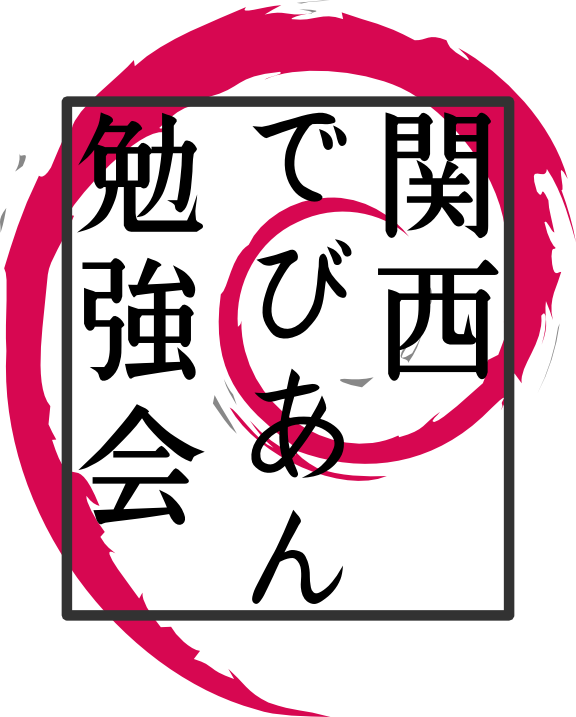
\includegraphics{image200802/kansaidebianlogo.png}
  \end{center}

  \begin{flushright}
    \hfill{}関西Debian勉強会担当者 佐々木・倉敷・のがた・かわだ \\
    \hfill{}\debmtgyear{}年\debmtgmonth{}月\debmtgdate{}日
  \end{flushright}

  \thispagestyle{empty}
\end{titlepage}

\dancersection{Introduction}{Debian JP}

\vspace{1em}

関西Debian勉強会はDebian GNU/Linuxのさまざまなトピック
(新しいパッケージ、Debian特有の機能の仕組、Debian界隈で起こった出来事、
などなど)について話し合う会です。

目的として次の三つを考えています。
\begin{itemize}
\item MLや掲示板ではなく、直接顔を合わせる事での情報交換の促進
\item 定期的に集まれる場所
\item 資料の作成
\end{itemize}

 それでは、楽しい一時をお過ごしください。

\newpage

\begin{minipage}[b]{0.2\hsize}
  {\rotatebox{90}{\fontsize{80}{80}
{\gt{関西 Debian 勉強会}}}}
\end{minipage}
\begin{minipage}[b]{0.8\hsize}
\hrule
\vspace{2mm}
\hrule
\setcounter{tocdepth}{1}
\tableofcontents
\vspace{2mm}
\hrule
\end{minipage}

\dancersection{最近のDebian関係のイベント報告}{Debian JP}

\subsection{第113回関西Debian勉強会@OSC 2016 Kyoto}

113回目の関西Debian勉強会は8月28日(日)に福島区民センターで開催されました。

内容はもくもくの会でしたが、飛び込みで syn さんの Enigma のお話しもありました。


\subsection{第143回東京エリアDebian勉強会}

143回目の東京エリアDebian勉強会は9月17日(土)に株式会社朝日ネットさんで開催されま
した。

内容は岩松さんによる「DEP5/Machine-readable debian/copyright 再考」でした。
debian/copyrigt の更新を手助けするツールとして licensecheck と licensecheck2dep5
や cme と libconfig-model-dpkg-perl、チェック用の license-reconcile などが紹介さ
れています。


\subsection{Debian Project}

\subsubsection{Updated Debian 8: 8.6 released}

Debian 8.6がリリースされました
\footnote{\url{https://lists.debian.org/debian-announce/2016/msg00008.html}}。


\subsubsection{Declassifying debian-private再び}

先日行なわれた「Declassifying debian-private
\footnote{\url{https://www.debian.org/vote/2016/vote_002}}」ですが、改正案の修正
が反映されていないまま投票が行なわれた
\footnote{\url{https://lists.debian.org/debian-vote/2016/09/msg00004.html}}とい
うことで再度GR「Declassifying debian-private
\footnote{\url{https://www.debian.org/vote/2016/vote_004}}」になりました。

僅差だった結果に対案も出ていますので、今回のGRで結果かわるかもしれません。


\subsubsection{Support for merged-/usr now in debootstrap; default for stretch?}

debootstrap 1.0.83で/usrディレクトリへのマージがサポートされました
\footnote{\url{https://lists.debian.org/debian-devel/2016/09/msg00269.html}}。

新しい--merged-usrオプションを追加して試してみてください。

\begin{commandline}
$ sudo debootstrap --merged-usr testing /path/to/debootstrap/root http://ftp.jp.debian.org/debian
\end{commandline}
%$


\subsubsection{Introducing default-mysql-* metapackages}

いくつかあるMySQL派生のデータベースのなかでMariaDBがデフォルトになりましたが、デ
フォルトの切り替えを容易にするためメタパッケージdefault-mysql-*が追加されました
\footnote{\url{https://lists.debian.org/debian-devel-announce/2016/09/msg00000.html}}。

default-mysql-serverパッケージをインストールするとmariadb-server-10.0パッケージ
がひっぱられてインストールされます。mysql-server-5.6がインストールされていると
MariaDBで置き換えられますがデータは移行されませんのでdump/importする必要がありま
す。

従来からあるvirtual-mysql-*とは用途が異なるものですのでこちらは引き続き提供され
ます。


\dancersection{事前課題}{関西Debian勉強会}

今回の事前課題はありませんでした。

参加者の皆さんは以下の通りです:

\begin{prework}{ lurdan }
\end{prework}

\begin{prework}{ t3rkwd }
\end{prework}

\begin{prework}{ むんくさん }
\end{prework}

\begin{prework}{ Yosuke OTSUKI }
\end{prework}

\begin{prework}{ 川江 浩 }
\end{prework}


\dancersection{初心者が初めてパッケージを作成してみた}{Yosuke OTSUKI}

\subsection{ Debian Package を作成する }

2016 年 9 月 23 日の時点で Debian 正式リリース版には 42612 のパッケージがあります。
これらのパッケージは、debian package maintainer (以下 maintainer) と debian developer (以下 developer)  と呼ばれるボランティアによって管理されています。
この記事は、debian maintainer になりたい初心者が初めて debian package を作成してみた手順を書き記しています。

\subsubsection{ 作成するパッケージを決める }

最初に作成すパッケージを決めます。
まだパッケージ化がされておらず、他の maintainer や developer がパッケージ化の作業をしていないか確認しておきましょう。
自分で書いたアプリじケーションやライブラリをパッケージ化することが最も簡単でしょう。
しかし、他の人が作成したソフトウェアを改造したり、使っているのであればそれらのソフトウェアをパッケージ化することを考えても良いかもしれません。
また、maintainer や developer の管理から外れたパッケージや、パッケージ化の要望が出ているソフトウェアをパッケージ化する手もあります。

今回の例では、maintainer や developer の管理から外れた orphan package と呼ばれるパッケージを引き取り mainter になってみましょう。

\begin{itemize}
    \item{ 自分で作成したものをパッケージ化する }
    \item{ 自分がよく使うパッケージを作成する }
    \item{ Orphan Package を引き取る \url{https://www.debian.org/devel/wnpp/orphaned}  }
    \item{ 改善が必要とされるパッケージ \url{https://www.debian.org/devel/wnpp/} }
\end{itemize}

自分がパッケージ化するソフトウェアの著作を持っている個人/団体を総称して upstream と呼びます。
もし自分が作成したソフトウェアならば、upstream も自分です。
ソフトウェアが debian の理念に従っていない場合、package mainter は upstream 側の開発者と交渉したり、
upstream 版を改修し、debian の独自バージョンを作成することがあります。

\subsubsection{ unstable 環境を整える }
パッケージを作成するための環境を整えます。 
パッケージの開発は、debian unstable で行わなければなりません。
2016 年 9 月現在の unstable は sid と呼ばれているバージョンです。

sid は開発者によって、日々機能追加や修正が行われています。
そのため、現在の安定版リリースを元に更新のあるパッケージを取り込むことで、最新の開発環境を整えます。
Debian の repository を jessie から sid に変更し、最新のパッケージリストに更新します。

\begin{commandline}
yosuke@ca200 # vi /etc/apt/sources.list

deb http://ftp.jaist.ac.jp/debian/ sid main
deb-src http://ftp.jaist.ac.jp/debian/ sid main
\end{commandline}

その後、パッケージリストを repository から取得しなおしてください。

\begin{commandline}
yosuke@ca200 # apt-get update 
yosuke@ca200 # apt-get upgrade
\end{commandline}

さらに、パッケージ開発に必要なツールをインストールします。
\begin{commandline}
yosuke@ca200 # apt-get install build-essentials debhelper devscripts cowdancer pbuilder 
\end{commandline}

以上で、開発環境が整いました。

\subsubsection{ パッケージを作成する }
今回は rc という shell パッケージをサンプルにパッケージ化の流れを説明したいと思います。
rc は orphan pakcage に掲載されています。\footnote{ rc は 2016/09/17 日現在 Orphan list にあるんですが、パッケージの更新がされています。これ、Debian あるあるなんでしょうか? }
rc を選んだ理由は、筆者がたまに使うことがある、実装をある程度読んだことがある、そして非常にシンプルなソフトウェア (外部ライブラリを使用しない) であるためです。

本来ならば、他の maintainer や developer に「自分が作業してるよー」と宣言する必要があります。
\footnote{宣言の種類は \url{https://www.debian.org/devel/wnpp/} }
しかし、今回作成した rc は練習なので、この作業をしません。

upstream の repository からソースコードを取得し、ソースコードを展開します。
dh\_make という、upstream のパッケージを debian かするためのコマンドを使用します。
まずは下準備をします。 テキストエディタで、.bashrc を編集し自分のメールアドレスと名前を下記のように記述してください。

\begin{commandline}
vi $HOME/.bashrc

DEBEMAIL="y.otsuki30 bug free At gmail.com"
DEBFULLNAME="Yosuke OTSUKI"
export DEBEMAIL DEBFULLNAME
\end{commandline}

作業用のディレクトリを作成し、その中で dh\_make を実行します。

\begin{commandline}
yosuke@debian-sid:$mkdir rc-1.7.4
yosuke@debian-sid:$ls . 
rc-1.7.4 rc-1.7.4.tar.gz
yosuke@debian-sid:$ cd rc-1.7.4 
yosuke@debian-sid:$ dh_make
Type of package: (single, indep, library, python)
[s/i/l/p]?
Email-Address       : y.otsuki30@gmail.com
License             : blank
Package Name        : rc
Maintainer Name     : Yosuke OTSUKI
Version             : 1.7.4
Package Type        : single
Date                : Fri, 23 Sep 2016 14:34:17 -0400
Are the details correct? [Y/n/q]

Could not find rc_1.7.4.orig.tar.xz
Either specify an alternate file to use with -f,
or add --createorig to create one.
\end{commandline}

このパッケージの場合、Type of package で single を選択します。
single は計算機アーキテクチャに依存性があるバイナリアプリケーションです。
indep は計算機アーキテクチャに依存性がないアプリケーション、library は共有ライブラリです。
python は文字通りだと思います。参照した資料が古く python に関しての言及がありませんでした。

正常終了すると、debian というディレクトリが生成されます。
\begin{commandline}
yosuke@debian-sid:~/Debian/rc2$ ls rc-1.7.4/debian/
changelog  manpage.1.ex     postinst.ex  rc.cron.d.ex    README.Debian  watch.ex
compat     manpage.sgml.ex  postrm.ex    rc.default.ex   README.source
control    manpage.xml.ex   preinst.ex   rc.doc-base.EX  rules
copyright  menu.ex          prerm.ex     rc-docs.docs    source
\end{commandline}

copyright ファイルにソフトウェアの著者の情報とライセンスを明記します。
\begin{commandline}
Format: http://www.debian.org/doc/packaging-manuals/copyright-format/1.0/
Upstream-Name: rc
Upstream-Contact: toby@paccrat.org
Souce: http://tobold.org/article/rc 

Files: rc-1.7.4/*
Copyright:  2016 Toby Goodwin,
            1991, 1999, 2001-2003, 2014, 2015 Byron Rakitzis,
            Paul Haahr
License: Zlib
\end{commandline}

changelog に変更の履歴を記載します。
今回は initial release とします。\footnote{本当は orphan なので、過去のバージョンからの更新情報が必要}
\begin{commandline}
rc-1.7.4 distribution: urgency=normal

    *Initial Release
        Sample packaging for 114th Kansai Debian Study 
    -- Yosuke OTSUKI yosuke30@gmail.com     2016/09/23
\end{commandline}

control を編集します。
\url{https://www.debian.org/doc/debian-policy/ch-archive.html#s-subsections} 
\begin{commandline}
Source: rc
Section: main
Priority: optional
Maintainer: Yosuke OTSUKI <y.otsuki30@gmail.com>
Build-Depends: debhelper (>= 9)
Standards-Version: 1.7.4
Homepage: http://tobold.org/article/rc 
#Vcs-Git: https://anonscm.debian.org/collab-maint/rc.git
#Vcs-Browser: https://anonscm.debian.org/cgit/collab-maint/rc.git
 
Package: rc
Architecture: x86_64
Depends:
Description: Plan 9 Shell
\end{commandline}

作業用のディレクトリで pbuilder によってパッケージを作成します。
\begin{commandline}
yosuke@debian-sid:# pbuilder create
yosuke@debian-sid:$ls ../
rc-1.7.4                  rc_1.7.4-1.debian.tar.xz  rc-1.7.4.tar.gz
rc_1.7.4-1_amd64.changes  rc_1.7.4-1.dsc
rc_1.7.4-1_amd64.deb      rc_1.7.4.orig.tar.gz
\end{commandline}

\subsubsection{ 参考資料 }
\begin{itemize}
    \item{\url{https://www.debian.org/doc/manuals/maint-guide/first.en.html} access date 2016/09/23 }
    \item{\url{https://wiki.debian.org/DebianMaintainer#Becoming_a_Debian_Maintainer} access date 2016/09/23 }
\end{itemize}

\subsection{ Maintainer になる (道なかば) }

Debian Projet の maintainer になるためには、他の maintainer や developer からの信頼を得なければなりません。
debian では、他の maintainer や developer と直接対面し、公的な写真付き身分証明書によって本人確認を行い、
自分の GPG キーに相手の GPG キーを登録してもらうことで、信頼を築ききます。
この一連の手順をキーサインをすると言います。
package maintainer になるためには、最低 1 人の Debian developer に鍵の登録をしてもらわなければなりません。
もし、知り合いに Debian developer がいない場合は、東京 Debian 勉強会や、関西 Debian 勉強会までいらしてください。
もしくは、Debian や Opensource 関連の大きなイベントで、大人数の鍵を交換と下集まりであるキーサインパーティなどに出席してみるのも手です。

\subsubsection{ GPG の鍵を作成する }

まず最初に自分の鍵を作成しなければなりません。
鍵の作成には、GNU Privacy Guard (以下 GPG ) というアプリケーションを使用します。
下記コマンドを使用して、GPG をインストールしましょう。
\begin{commandline}
yosuke@ca200 $ sudo apt-get instal gpg
\end{commandline}

鍵の作成の前に、すでに鍵がないか確認しておきます。
\$HOME 以下に、GPG のディレクトリが作成されます。 すでに存在している鍵は上書きされるので注意が必要です。
もし存在するのならば、バックアップを取っておきましょう。
\begin{commandline}
yosuke@ca_200 $ ls $HOME/.gnupg 
\end{commandline}

鍵の作成をします。
\begin{commandline}
yosuke@ca200 $ gpg --gen-key
\end{commandline}

\subsubsection{ GPG の鍵を public key server に登録する }

自分の鍵を作成したら、鍵を公開鍵サーバーに登録します。
こうすることで、世界中のインターネットユーザーの中から個人を特定するとこができます。
そのため、自分の鍵の保管には非常に注意を払わなければなりません。

\begin{commandline}
yosuke@ca200 $ gpg --keyserver keyring.debian.org --send-key 84D1A6F2
\end{commandline}

84D1A6F2 は筆者のキー ID です。

\subsubsection{ キーサインをする }
キーサインをしてもらいに行きましょう。
以下のように自分のキーを紙に印刷して、短冊のように切ってください。
大体 A4 の印刷用紙から 8 個程度作成できるはずです。

\begin{commandline}
yosuke@ca200 $ gpg --fingerprint
/home/yosuke/.gnupg/pubring.gpg
-------------------------------
pub   4096R/84D1A6F2 2016-08-28
      Key fingerprint = 310C 6FCE 254A E0DF 395D  23A3 D2F2 5C56 84D1 A6F2
uid                  Yosuke OTSUKI (Yosuke's personal key) <y.otsuki30@gmail.com>
sub   4096R/F6F3EC9D 2016-08-28
\end{commandline}

他に、キーサインをするために、写真付きの公的機関が発行した身分証明書が必要です。
日本語がわかる人ならば、運転免許証がなどで事足りますが、
海外の方とキーサインする可能性があるのならば、パスポートの用意もしておいたほうが良いかもしれません。

キーサインの場では、あなたのキーをキーを交換する相手に渡してください。そして、身分証明書を相手に提示します。
相手から身分証明証を受け取ったらば、本人であるか確認し、相手の鍵の書かれた用紙を受け取ってください。

相手の鍵が書かれている紙を受け取ったらば、自分の鍵の登録します。

公開鍵サーバーから相手の鍵を受け取ります。
ここでは、相手の鍵が 00AA11BB とします。
\begin{commandline}
yosuke@ca200 $ gpg --recv-keys 00AA11BB
\end{commandline}

自分の鍵に相手の鍵をサインします。
\begin{commandline}
yosuke@ca200 $ gpg --sign-key 00AA11BB
\end{commandline}

自分がサインした鍵を相手に送るため出力します。

\begin{commandline}
yosuke@ca200 $ gpg --armor --output 00AA11BB-signedBy-84D1A6F2.asc --export 00AA11BB
\end{commandline}

相手がキーサインした鍵を受け取ったらば、自分の鍵に取り込みます。

\begin{commandline}
yosuke@ca200 $ gpg --import 84D1A6F2-signedBy-00AA11BB.asc 
\end{commandline}

そして、公開鍵サーバーの鍵を更新すれば完了です。

\begin{commandline}
yosuke@ca200 $ gpg --send 84D1A6F2 
\end{commandline}

\subsubsection{ 参考資料 }
\url{https://wiki.debian.org/Keysigningi} access date 2016/09/23


\dancersection{Let's Encrypt のススメ}{かわだ てつたろう}

\subsection{はじめに}

無料でSSL/TLS証明書を取得できるサービスとしてStart SSLやWo Sign、CAcertなどいく
つかありますが、今回はDebianパッケージを使用して簡単に導入できるLet's Encryptを
紹介します。


\subsection{Let's Encryptについて}

Let's Encrypt\footnote{\url{https://letsencrypt.org/}}は2016年4月12日にサービス
を開始した認証局(CA)です。日本語の情報は「Let's Encrypt 総合ポータル
\footnote{\url{https://letsencrypt.jp/}}」にまとまっていますので参照してください。

その特徴として
\begin{itemize}
\item フリーで自動化されたオープンな認証局
\item 非営利団体ISRG(Internet Security Research Group)が運営
\item ACME(Automated Certificate Management Environment)プロトコル
\end{itemize}
があげられます。

\subsubsection{証明書}

発行される証明書は、ドメイン認証(DV:Domain Validation)証明書です。
企業認証(OV:Organization Validation)証明書やEV(Extended Validation)証明書は発行
されません。ワイルドカード証明書には対応していませんが、複数のサブドメイン名の証
明書が取得できますので問題にはならないでしょう。

ルート証明書は、IdenTrust社の証明書(DST Root CA X3)でクロス署名されておりほとん
どの環境に対応しています
\footnote{\url{https://community.letsencrypt.org/t/which-browsers-and-operating-systems-support-lets-encrypt/4394}}
。DebianではDebian 6 squeezeから使用できます。

証明書の期限は90日となっており、60日ごとの更新がすすめられています
\footnote{\url{https://letsencrypt.org/2015/11/09/why-90-days.html}}。

\subsubsection{ACME}

ドメイン認証証明書発行にはドメイン所有者の確認が必要です。多くの場合その確認にCA
から送られてきたテキストを
\begin{itemize}
\item 対象ドメインのWebサーバで公開
\item 対象ドメインのDNSのTXTレコードに追加
\item 対象ドメインのメールアドレスで受けとりCAのWebページに入力
\end{itemize}
するなどドメイン所有者にしかできないいずれかの方法が取られます。

このようなドメイン所有者の確認を含めたCSRの作成から証明書発行までの手順を自動化し
標準化した仕様がACME\footnote{\url{https://github.com/ietf-wg-acme/acme/}}
になります。仕様はサーバ、クライアント両方について規定されており、Let's Encrypt
はサーバ側のリファレンス実装といえます。

ACMEでは次のいずれかの方法でドメイン所有者の確認が行なわれます。
\begin{itemize}
\item 対象ドメインのサーバでTLSを有効
\item 対象ドメインのDNSのTXTレコードに指定したテキストを追加
\item 対象ドメインのWebサーバで指定したテキストを公開
\end{itemize}

\subsection{導入}

それでは、実際にLet's Encryptの証明書を取得します。
環境は、DNSの設定は完了しているDebian 8.6 jessieで行ないます。また、事前に利用規
約\footnote{\url{https://letsencrypt.org/repository/}}を読んで同意しておいてくだ
さい。利用規約に同意したものとして手順を紹介します。

\subsubsection{certbot}

ACMEのクライアントアプリがDebianではcertbotパッケージとして提供されています。
jessieではjessie-backportsに含まれていますのでbackportsを有効にしてインストール
します。

\begin{commandline}
$ sudo -c 'echo deb http://ftp.jp.debian.org/debian jessie-backports main >> /etc/apt/source.list'
$ sudo apt update
$ sudo apt install certbot -t jessie-backports
\end{commandline}
%%$

\subsubsection{証明書取得}

証明書を取得するには次のコマンドを実行します。Webサーバ(ポート80と443を使用して
いるプロセス)を止めておいてください。

\begin{commandline}
$ sudo certbot certonly --standalone --agree-tos -m postmaster@example.org -d example.org
IMPORTANT NOTES:
 - Congratulations! Your certificate and chain have been saved at
   /etc/letsencrypt/live/example.org/fullchain.pem. Your cert will expire
   on 2016-12-23. To obtain a new or tweaked version of this
   certificate in the future, simply run certbot again. To
   non-interactively renew *all* of your certificates, run "certbot
   renew"
 - If you like Certbot, please consider supporting our work by:

   Donating to ISRG / Let's Encrypt:   https://letsencrypt.org/donate
   Donating to EFF:                    https://eff.org/donate-le
\end{commandline}
%$

これでexample.orgドメインの証明書が取得でき、/etc/letsencrypt/live/example.org
以下にcert.pem, chain.pem, fullchain.pem,privkey.pemができあがります。これらファ
イルをWebサーバなどに設定してSSL/TLSを有効にします。ファイルは
/etc/letsencrypt/archive/example.org以下の世代ファイルへのシンボリックリンクとなっ
ており、証明書を更新しても参照側の設定変更の必要をなくしています。

\subsubsection{webrootの使用}

多くの環境ではWebサーバが稼動しているはずです。証明書取得の度にWebサーバを止める
わけにはいきませんので、稼動しているWebサーバを利用してドメイン所有の確認を行な
うwebrootオプションを使うことになります。

複数のドメイン、サブドメインを使用する場合はドメインごとにwebrootの設定を行なう
ことになりますが、これを一つのディレクトリにまとめる方法がArch Wikiに記載されて
います\footnote{\url{https://wiki.archlinux.org/index.php?title=Let\%E2\%80\%99s_Encrypt}}。

これを利用してnginx環境で行なうと次のようになります。

\begin{commandline}
$ cat /etc/nginx/snippets/letsencrypt.conf
location ^~ /.well-known/acme-challenge {
    alias /var/lib/letsencrypt/.well-known/acme-challenge;
    default_type "text/plain";
    try_files $uri =404;
}
$ cat /etc/nginx/sites-enabled/default
server {
  ...
  include /etc/nginx/snippets/letsencrypt.conf;
}
$ sudo certbot certonly --webroot --agree-tos -m postmaster@example.org -d example.org --hsts -w /var/lib/letsencrypt/
\end{commandline}

\subsubsection{証明書の更新}

証明書の更新はrenewで行ないます。

\begin{commandline}
$ sudo certbot renew
\end{commandline}
%$

更新は、証明書取得時に生成される/etc/letsencrypt/renewalの設定ファイルに従って行
なわれます。

Let's Encryptでは1日2回証明書の更新を行なうことが推奨されています。Debianパッケー
ジには/etc/cron.d/certbotが含まれておりインストールした時点で行なうようになって
います。

証明書は期限が指定期日(デフォルト30日)未満になると更新されますが、更新された場合
Webサーバなど使用しているサービスの再起動などが必要です。そのためのオプションと
して--post-hockがありますので/etc/cron.d/certbotに指定しておくとよいでしょう。

\subsubsection{その他}

certbotのデフォルトサブコマンドrunでは証明書の取得からWebサーバへのインストール
までを行います。筆者はWebサーバの設定ファイルまで書き換えるのは望まないので使用
しませんでした。nginxには対応途中のようですがApacheをお使いの方は試されてみると
よいでしょう。

その他に証明書の失効などさまざまなこともcertbotコマンドで行なえますので詳しくは
ドキュメント\footnote{\url{https://certbot.eff.org/docs/}}してください。


\subsection{まとめ}

Let's Encryptの紹介とcertbotを使った証明書の取得、更新の仕方について説明しました。
手軽に証明書の取得が行なえますのでぜひ導入して暗号化しましょう。ただし、期限の短
い証明書になりますので、自動更新設定をきっちり行なって期限切れにならないよう気を
つけてください。


\dancersection{今後の予定}{Debian JP}

\subsection{関西Debian勉強会}
次回、第115回関西Debian勉強会は10月24(日)に開催予定です。

\subsection{東京エリアDebian勉強会}
次回、第144回東京エリアDebian勉強会は10月15日(土)に開催予定です。

%
% 冊子にするために、4の倍数にする必要がある。
% そのための調整
\dancersection{メモ}{}
\mbox{}\newpage
\mbox{}\newpage
% \mbox{}\newpage

\pagebreak

\begin{center}
本資料のライセンスについて
\end{center}

本資料はフリー・ソフトウェアです。あなたは、Free Software
Foundation が公表したGNU GENERAL PUBLIC LICENSEの "バージョン2"もしくはそれ以降
が定める条項に従って本プログラムを再頒布または変更することができ
ます。

本プログラムは有用とは思いますが、頒布にあたっては、市場性及び特
定目的適合性についての暗黙の保証を含めて、いかなる保証も行ないま
せん。詳細についてはGNU GENERAL PUBLIC LICENSE をお読みください。

\begin{multicols}{2}
 \begin{fontsize}{6}{6}
 \begin{verbatim}
            GNU GENERAL PUBLIC LICENSE
               Version 2, June 1991

 Copyright (C) 1989, 1991 Free Software Foundation, Inc.
    51 Franklin St, Fifth Floor, Boston, MA  02110-1301  USA
 Everyone is permitted to copy and distribute verbatim copies
 of this license document, but changing it is not allowed.

                Preamble

  The licenses for most software are designed to take away your
freedom to share and change it.  By contrast, the GNU General Public
License is intended to guarantee your freedom to share and change free
software--to make sure the software is free for all its users.  This
General Public License applies to most of the Free Software
Foundation's software and to any other program whose authors commit to
using it.  (Some other Free Software Foundation software is covered by
the GNU Library General Public License instead.)  You can apply it to
your programs, too.

  When we speak of free software, we are referring to freedom, not
price.  Our General Public Licenses are designed to make sure that you
have the freedom to distribute copies of free software (and charge for
this service if you wish), that you receive source code or can get it
if you want it, that you can change the software or use pieces of it
in new free programs; and that you know you can do these things.

  To protect your rights, we need to make restrictions that forbid
anyone to deny you these rights or to ask you to surrender the rights.
These restrictions translate to certain responsibilities for you if you
distribute copies of the software, or if you modify it.

  For example, if you distribute copies of such a program, whether
gratis or for a fee, you must give the recipients all the rights that
you have.  You must make sure that they, too, receive or can get the
source code.  And you must show them these terms so they know their
rights.

  We protect your rights with two steps: (1) copyright the software, and
(2) offer you this license which gives you legal permission to copy,
distribute and/or modify the software.

  Also, for each author's protection and ours, we want to make certain
that everyone understands that there is no warranty for this free
software.  If the software is modified by someone else and passed on, we
want its recipients to know that what they have is not the original, so
that any problems introduced by others will not reflect on the original
authors' reputations.

  Finally, any free program is threatened constantly by software
patents.  We wish to avoid the danger that redistributors of a free
program will individually obtain patent licenses, in effect making the
program proprietary.  To prevent this, we have made it clear that any
patent must be licensed for everyone's free use or not licensed at all.

  The precise terms and conditions for copying, distribution and
modification follow.

            GNU GENERAL PUBLIC LICENSE
   TERMS AND CONDITIONS FOR COPYING, DISTRIBUTION AND MODIFICATION

  0. This License applies to any program or other work which contains
a notice placed by the copyright holder saying it may be distributed
under the terms of this General Public License.  The "Program", below,
refers to any such program or work, and a "work based on the Program"
means either the Program or any derivative work under copyright law:
that is to say, a work containing the Program or a portion of it,
either verbatim or with modifications and/or translated into another
language.  (Hereinafter, translation is included without limitation in
the term "modification".)  Each licensee is addressed as "you".

Activities other than copying, distribution and modification are not
covered by this License; they are outside its scope.  The act of
running the Program is not restricted, and the output from the Program
is covered only if its contents constitute a work based on the
Program (independent of having been made by running the Program).
Whether that is true depends on what the Program does.

  1. You may copy and distribute verbatim copies of the Program's
source code as you receive it, in any medium, provided that you
conspicuously and appropriately publish on each copy an appropriate
copyright notice and disclaimer of warranty; keep intact all the
notices that refer to this License and to the absence of any warranty;
and give any other recipients of the Program a copy of this License
along with the Program.

You may charge a fee for the physical act of transferring a copy, and
you may at your option offer warranty protection in exchange for a fee.

  2. You may modify your copy or copies of the Program or any portion
of it, thus forming a work based on the Program, and copy and
distribute such modifications or work under the terms of Section 1
above, provided that you also meet all of these conditions:

    a) You must cause the modified files to carry prominent notices
    stating that you changed the files and the date of any change.

    b) You must cause any work that you distribute or publish, that in
    whole or in part contains or is derived from the Program or any
    part thereof, to be licensed as a whole at no charge to all third
    parties under the terms of this License.

    c) If the modified program normally reads commands interactively
    when run, you must cause it, when started running for such
    interactive use in the most ordinary way, to print or display an
    announcement including an appropriate copyright notice and a
    notice that there is no warranty (or else, saying that you provide
    a warranty) and that users may redistribute the program under
    these conditions, and telling the user how to view a copy of this
    License.  (Exception: if the Program itself is interactive but
    does not normally print such an announcement, your work based on
    the Program is not required to print an announcement.)

These requirements apply to the modified work as a whole.  If
identifiable sections of that work are not derived from the Program,
and can be reasonably considered independent and separate works in
themselves, then this License, and its terms, do not apply to those
sections when you distribute them as separate works.  But when you
distribute the same sections as part of a whole which is a work based
on the Program, the distribution of the whole must be on the terms of
this License, whose permissions for other licensees extend to the
entire whole, and thus to each and every part regardless of who wrote it.

Thus, it is not the intent of this section to claim rights or contest
your rights to work written entirely by you; rather, the intent is to
exercise the right to control the distribution of derivative or
collective works based on the Program.

In addition, mere aggregation of another work not based on the Program
with the Program (or with a work based on the Program) on a volume of
a storage or distribution medium does not bring the other work under
the scope of this License.

  3. You may copy and distribute the Program (or a work based on it,
under Section 2) in object code or executable form under the terms of
Sections 1 and 2 above provided that you also do one of the following:

    a) Accompany it with the complete corresponding machine-readable
    source code, which must be distributed under the terms of Sections
    1 and 2 above on a medium customarily used for software interchange; or,

    b) Accompany it with a written offer, valid for at least three
    years, to give any third party, for a charge no more than your
    cost of physically performing source distribution, a complete
    machine-readable copy of the corresponding source code, to be
    distributed under the terms of Sections 1 and 2 above on a medium
    customarily used for software interchange; or,

    c) Accompany it with the information you received as to the offer
    to distribute corresponding source code.  (This alternative is
    allowed only for noncommercial distribution and only if you
    received the program in object code or executable form with such
    an offer, in accord with Subsection b above.)

The source code for a work means the preferred form of the work for
making modifications to it.  For an executable work, complete source
code means all the source code for all modules it contains, plus any
associated interface definition files, plus the scripts used to
control compilation and installation of the executable.  However, as a
special exception, the source code distributed need not include
anything that is normally distributed (in either source or binary
form) with the major components (compiler, kernel, and so on) of the
operating system on which the executable runs, unless that component
itself accompanies the executable.

If distribution of executable or object code is made by offering
access to copy from a designated place, then offering equivalent
access to copy the source code from the same place counts as
distribution of the source code, even though third parties are not
compelled to copy the source along with the object code.

  4. You may not copy, modify, sublicense, or distribute the Program
except as expressly provided under this License.  Any attempt
otherwise to copy, modify, sublicense or distribute the Program is
void, and will automatically terminate your rights under this License.
However, parties who have received copies, or rights, from you under
this License will not have their licenses terminated so long as such
parties remain in full compliance.

  5. You are not required to accept this License, since you have not
signed it.  However, nothing else grants you permission to modify or
distribute the Program or its derivative works.  These actions are
prohibited by law if you do not accept this License.  Therefore, by
modifying or distributing the Program (or any work based on the
Program), you indicate your acceptance of this License to do so, and
all its terms and conditions for copying, distributing or modifying
the Program or works based on it.

  6. Each time you redistribute the Program (or any work based on the
Program), the recipient automatically receives a license from the
original licensor to copy, distribute or modify the Program subject to
these terms and conditions.  You may not impose any further
restrictions on the recipients' exercise of the rights granted herein.
You are not responsible for enforcing compliance by third parties to
this License.

  7. If, as a consequence of a court judgment or allegation of patent
infringement or for any other reason (not limited to patent issues),
conditions are imposed on you (whether by court order, agreement or
otherwise) that contradict the conditions of this License, they do not
excuse you from the conditions of this License.  If you cannot
distribute so as to satisfy simultaneously your obligations under this
License and any other pertinent obligations, then as a consequence you
may not distribute the Program at all.  For example, if a patent
license would not permit royalty-free redistribution of the Program by
all those who receive copies directly or indirectly through you, then
the only way you could satisfy both it and this License would be to
refrain entirely from distribution of the Program.

If any portion of this section is held invalid or unenforceable under
any particular circumstance, the balance of the section is intended to
apply and the section as a whole is intended to apply in other
circumstances.

It is not the purpose of this section to induce you to infringe any
patents or other property right claims or to contest validity of any
such claims; this section has the sole purpose of protecting the
integrity of the free software distribution system, which is
implemented by public license practices.  Many people have made
generous contributions to the wide range of software distributed
through that system in reliance on consistent application of that
system; it is up to the author/donor to decide if he or she is willing
to distribute software through any other system and a licensee cannot
impose that choice.

This section is intended to make thoroughly clear what is believed to
be a consequence of the rest of this License.

  8. If the distribution and/or use of the Program is restricted in
certain countries either by patents or by copyrighted interfaces, the
original copyright holder who places the Program under this License
may add an explicit geographical distribution limitation excluding
those countries, so that distribution is permitted only in or among
countries not thus excluded.  In such case, this License incorporates
the limitation as if written in the body of this License.

  9. The Free Software Foundation may publish revised and/or new versions
of the General Public License from time to time.  Such new versions will
be similar in spirit to the present version, but may differ in detail to
address new problems or concerns.

Each version is given a distinguishing version number.  If the Program
specifies a version number of this License which applies to it and "any
later version", you have the option of following the terms and conditions
either of that version or of any later version published by the Free
Software Foundation.  If the Program does not specify a version number of
this License, you may choose any version ever published by the Free Software
Foundation.

  10. If you wish to incorporate parts of the Program into other free
programs whose distribution conditions are different, write to the author
to ask for permission.  For software which is copyrighted by the Free
Software Foundation, write to the Free Software Foundation; we sometimes
make exceptions for this.  Our decision will be guided by the two goals
of preserving the free status of all derivatives of our free software and
of promoting the sharing and reuse of software generally.

                NO WARRANTY

  11. BECAUSE THE PROGRAM IS LICENSED FREE OF CHARGE, THERE IS NO WARRANTY
FOR THE PROGRAM, TO THE EXTENT PERMITTED BY APPLICABLE LAW.  EXCEPT WHEN
OTHERWISE STATED IN WRITING THE COPYRIGHT HOLDERS AND/OR OTHER PARTIES
PROVIDE THE PROGRAM "AS IS" WITHOUT WARRANTY OF ANY KIND, EITHER EXPRESSED
OR IMPLIED, INCLUDING, BUT NOT LIMITED TO, THE IMPLIED WARRANTIES OF
MERCHANTABILITY AND FITNESS FOR A PARTICULAR PURPOSE.  THE ENTIRE RISK AS
TO THE QUALITY AND PERFORMANCE OF THE PROGRAM IS WITH YOU.  SHOULD THE
PROGRAM PROVE DEFECTIVE, YOU ASSUME THE COST OF ALL NECESSARY SERVICING,
REPAIR OR CORRECTION.

  12. IN NO EVENT UNLESS REQUIRED BY APPLICABLE LAW OR AGREED TO IN WRITING
WILL ANY COPYRIGHT HOLDER, OR ANY OTHER PARTY WHO MAY MODIFY AND/OR
REDISTRIBUTE THE PROGRAM AS PERMITTED ABOVE, BE LIABLE TO YOU FOR DAMAGES,
INCLUDING ANY GENERAL, SPECIAL, INCIDENTAL OR CONSEQUENTIAL DAMAGES ARISING
OUT OF THE USE OR INABILITY TO USE THE PROGRAM (INCLUDING BUT NOT LIMITED
TO LOSS OF DATA OR DATA BEING RENDERED INACCURATE OR LOSSES SUSTAINED BY
YOU OR THIRD PARTIES OR A FAILURE OF THE PROGRAM TO OPERATE WITH ANY OTHER
PROGRAMS), EVEN IF SUCH HOLDER OR OTHER PARTY HAS BEEN ADVISED OF THE
POSSIBILITY OF SUCH DAMAGES.

             END OF TERMS AND CONDITIONS

        How to Apply These Terms to Your New Programs

  If you develop a new program, and you want it to be of the greatest
possible use to the public, the best way to achieve this is to make it
free software which everyone can redistribute and change under these terms.

  To do so, attach the following notices to the program.  It is safest
to attach them to the start of each source file to most effectively
convey the exclusion of warranty; and each file should have at least
the "copyright" line and a pointer to where the full notice is found.

    <one line to give the program's name and a brief idea of what it does.>
    Copyright (C) <year>  <name of author>

    This program is free software; you can redistribute it and/or modify
    it under the terms of the GNU General Public License as published by
    the Free Software Foundation; either version 2 of the License, or
    (at your option) any later version.

    This program is distributed in the hope that it will be useful,
    but WITHOUT ANY WARRANTY; without even the implied warranty of
    MERCHANTABILITY or FITNESS FOR A PARTICULAR PURPOSE.  See the
    GNU General Public License for more details.

    You should have received a copy of the GNU General Public License
    along with this program; if not, write to the Free Software
    Foundation, Inc., 51 Franklin St, Fifth Floor, Boston, MA  02110-1301 USA


Also add information on how to contact you by electronic and paper mail.

If the program is interactive, make it output a short notice like this
when it starts in an interactive mode:

    Gnomovision version 69, Copyright (C) year  name of author
    Gnomovision comes with ABSOLUTELY NO WARRANTY; for details type `show w'.
    This is free software, and you are welcome to redistribute it
    under certain conditions; type `show c' for details.

The hypothetical commands `show w' and `show c' should show the appropriate
parts of the General Public License.  Of course, the commands you use may
be called something other than `show w' and `show c'; they could even be
mouse-clicks or menu items--whatever suits your program.

You should also get your employer (if you work as a programmer) or your
school, if any, to sign a "copyright disclaimer" for the program, if
necessary.  Here is a sample; alter the names:

  Yoyodyne, Inc., hereby disclaims all copyright interest in the program
  `Gnomovision' (which makes passes at compilers) written by James Hacker.

  <signature of Ty Coon>, 1 April 1989
  Ty Coon, President of Vice

This General Public License does not permit incorporating your program into
proprietary programs.  If your program is a subroutine library, you may
consider it more useful to permit linking proprietary applications with the
library.  If this is what you want to do, use the GNU Library General
Public License instead of this License.
 \end{verbatim}
 \end{fontsize}
\end{multicols}

\begin{center}
ソースコードについて
\end{center}

このプログラムは tex で記述されたものです。ソースコードは
\begin{center}
  \url{git://anonscm.debian.org/tokyodebian/monthly-report.git}
\end{center}
から取得できます。

\begin{center}
Debian オープンユーズロゴ ライセンス
\end{center}

\begin{multicols}{2}
 \begin{fontsize}{6}{6}
 \begin{verbatim}

Copyright (c) 1999 Software in the Public Interest
Permission is hereby granted, free of charge, to any person
obtaining a copy of this software and associated documentation
files (the "Software"), to deal in the Software without restriction,
including without limitation the rights to use, copy, modify, merge,
publish, distribute, sublicense, and/or sell copies of the Software,
and to permit persons to whom the Software is furnished to do so,
subject to the following conditions:

The above copyright notice and this permission notice shall be
included in all copies or substantial portions of the Software.

THE SOFTWARE IS PROVIDED "AS IS", WITHOUT WARRANTY OF ANY
KIND, EXPRESS OR IMPLIED, INCLUDING BUT NOT LIMITED TO THE
WARRANTIES OF MERCHANTABILITY, FITNESS FOR A PARTICULAR PURPOSE AND
NONINFRINGEMENT. IN NO EVENT SHALL THE AUTHORS OR COPYRIGHT HOLDERS
BE LIABLE FOR ANY CLAIM, DAMAGES OR OTHER LIABILITY, WHETHER IN
AN ACTION OF CONTRACT, TORT OR OTHERWISE, ARISING FROM, OUT OF OR
IN CONNECTION WITH THE SOFTWARE OR THE USE OR OTHER DEALINGS IN
THE SOFTWARE.
 \end{verbatim}
 \end{fontsize}
\end{multicols}

\printindex
%\cleartooddpage

 \begin{minipage}[b]{0.2\hsize}
  \rotatebox{90}{\fontsize{80}{80} {\gt 関西 Debian 勉強会} }
 \end{minipage}
 \begin{minipage}[b]{0.8\hsize}

 \vspace*{15cm}
 \rule{\hsize}{1mm}
 \vspace{2mm}
 
\includegraphics[width=2cm]{image200502/openlogo-nd.eps}
 \noindent \Large \bfseries{Debian 勉強会資料}\\ \\
 \noindent \normalfont \debmtgyear{}年\debmtgmonth{}月\debmtgdate{}日 \hspace{5mm}  初版第1刷発行\\
 \noindent \normalfont 関西 Debian 勉強会 (編集・印刷・発行)\\
 \rule{\hsize}{1mm}
 \end{minipage}

\end{document}
%%% Local Variables:
%%% skk-kutouten-type: jp
%%% End:
